\section{Results and discussion}
In this study, the algorithms DT, RF, LR, NB, SVM and ANN were applied on five datasets concerning patients with or without malaria and living in regions of Senegal namely: Diourbel, Thies and Fatick. Indeed, in order to offer a new technique for diagnosing and predicting malaria, it is important to know the performance of those existing through our datasets.\\
Table \ref{raw_data1} presents the results of the experiments with the different algorithms on our data on Malaria. More specifically, Table 2 contains the precision, the recall, the specificity, the AUC mesure, the score and F-measure of each algorithm tested while Figure 1 shows their respective ROC curve.  
\begin{table}[h]
\begin{tabular}{|l|c|c|c|c|c|c|c|}
\hline
\cline{2-8}
 \textbf{ML ALgorithms} &  \textbf{Datasets} & \textbf{Precision} & \textbf{Recall} & \textbf{F1-score}&\textbf{AUC} &\textbf{Score}&\textbf{Specificity}\tabularnewline
\hline
\cline{2-8}
 &  DT1 &0.97  & 1   & 0.98 & 0.78 & 97.04 & 0.05 \\
\cline{2-8}
& DT2 & 0.59 &0.48 &0.48  &0.64  &63.01  &0.80\\
\cline{2-8}
& DT3 &0.89  &0.85 &0.87  &0.86  &80.86  &0.69\\
\cline{2-8}
& DT4 &0.68  &0.57 &0.62  &0.70  &65.60  &0.74\\
\cline{2-8}
\multirow{-4}{*}{ \textbf{Decision Tree}}&   DT5 &0.99  &0.84 &0.91  &0.76  &83.41  &0.58\\
\hline
\cline{2-8}
&DT1 &0.97 &1   &0.99 &0.81 &97.13& 0.07\\
\cline{2-8}
 & DT2 &0.63  & 0.34  &0.44&0.64&63.33& 0.85\\
 \cline{2-8}
 & DT3 &0.89 &0.85 &0.87&087&80.86&0.70\\
 \cline{2-8}
 & DT4 &0.68 &0.56&0.62&0.70&65.82&0.74\\
\cline{2-8}
\multirow{-4}{*}{ \textbf{Random Forest}}&   DT5 &0.99 &0.84&0.91&0.76&78.35&0.60\\
\hline
\cline{2-8}
&DT1 &0.97 &1   &0.99 &0.79 &97.19&0.05 \\
\cline{2-8}
 &DT2 & 0.58 &0.36   &0.44&0.63&61.96&0.81\\
 \cline{2-8}
  &DT3 &0.85 &0.88 &0.86&0.86&79.59&0.55\\
  \cline{2-8}
  &DT4 &0.98 &0.56&0.92&0.70&65.82&0.72\\
  \cline{2-8}
\multirow{-4}{*}{ \textbf{Logistic Regression}}&   DT5 & 0.90&0.78&0.88&0.84&81.86&0.75\\
\hline
\cline{2-8}
& DT1 &0.97 &1   &0.99 &0.81 &97.13 &0.00\\
 \cline{2-8}
  &DT2 & 0.60 &0.34   &0.43&0.63&62.86&0.83 \\
  \cline{2-8}
  &DT3 &0.86 &0.87 &0.86&0.85&79.94&0.60\\
  \cline{2-8}
  &DT4 &0.68 &0.59&0.63&0.70&65.63&0.73\\
  \cline{2-8}
\multirow{-4}{*}{ \textbf{Naive Bays}}&0.99 &0.82&0.90&0.84&85.61&0.71&0.71\\
\hline
\cline{2-8}
&DT1 &0.97 &1   &0.99 &0.84 &97.13&0.00 \\
\cline{2-8}
  &DT2 &0.58  &0.05   & 0.09&0.62&62.86&0.97\\
  \cline{2-8}
  &DT3 &0.57 & 0.86&0.86&0.85&79.94&0.64\\
  \cline{2-8}
 & DT4 & 0.68&0.58&0.62&0.70&65.63&0.73\\
 \cline{2-8}
 \multirow{-4}{*}{ \textbf{Support V Machine}}& DT5 &0.99 &0.86&0.92&0.80&85.61&0.62\\
 \hline
\cline{2-8}
&DT1 &0.97&1 &0.99   &0.84 &97.15&0.04  \\
\cline{2-8}
&  DT2 &0.59  &0.40   &0.48&0.65&62.86&0.80 \\
\cline{2-8}
 & DT3 &0.89 &0.85 &0.87&0.87&86.68&0.69\\
 \cline{2-8}
 & DT4 &0.68 &0.58&0.62&0.70&0.70&0.75\\
  \cline{2-8}
  \multirow{-4}{*}{ \textbf{ Artificial N Network}}&DT5 &0.99 &0.84&0.91&0.79&83.26&0.65\\ 
  \hline
\end{tabular}
\caption{Performances measures of our classifiers over all datasets}\label{raw_data1}
\end{table}
\\
Analysing in details the performance of our six classifiers across the five datasets, the results show that there is not necessarily a single best classification algorithm, but that the best performing algorithm will depend on the characteristics of the dataset to analyze. Indeed we notice that all the algorithms produce their best precision on the DT1, DT3, and DT5 data sets. These values, which reach 97\% at times, outperform the Rapid Diagnosis Test which is the standard diagnostic tool largely adopted in the healthcare system in Senegal.
\begin{figure}[h]
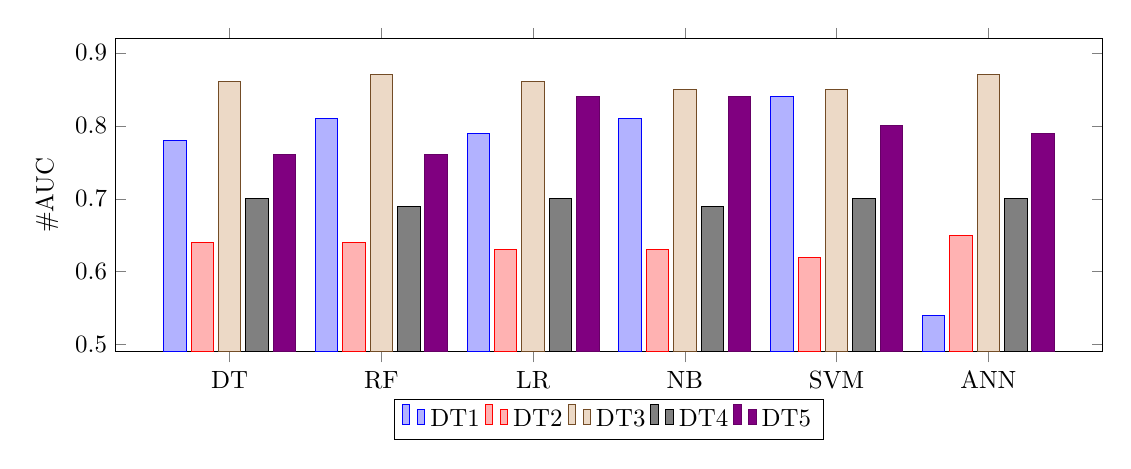
\begin{tikzpicture}[scale=0.9]
 \centering
\begin{axis}[
    height=6cm, width=15.5cm,
    bar width=0.4cm,
    ybar,
    %ybar=5pt,% configures `bar shift'
    bar width=9pt,
    enlargelimits=0.15,
    legend style={at={(0.5,-0.15)},
    anchor=north,legend columns=-1},
    ylabel={\#AUC},
    symbolic x coords={{DT,RF,LR,NB,SVM,ANN}},
    xtick=data,
    %nodes near coords,
    nodes near coords align={vertical},
    ]
\addplot coordinates {(DT,0.78) (RF, 0.81) (LR,0.79)(NB, 0.81)(SVM,0.84)(ANN, 0.54)};
\addplot coordinates{(DT,0.64) (RF, 0.64) (LR,0.63)(NB, 0.63)(SVM,0.62)(ANN, 0.65)};
\addplot coordinates {(DT,0.86) (RF, 0.87) (LR,0.86)(NB, 0.85)(SVM,0.85)(ANN, 0.87)};
\addplot coordinates {(DT,0.70) (RF, 0.69) (LR,0.70)(NB, 0.69)(SVM,0.70)(ANN, 0.70)};
\addplot coordinates {(DT,0.76) (RF, 0.76) (LR,0.84)(NB, 0.84)(SVM,0.80)(ANN, 0.79)};
\legend{DT1,DT2,DT3,DT4,DT5}
\end{axis}
\end{tikzpicture}
\caption{Comparison of the ROC Curves of the classifiers on differents datasets}
\end{figure}
However, on these same datasets, the algorithms often present very low specificities, for example 0.05 on DT1. This shows that our best performing classifiers are only able to predict a single class: either the patient has malaria or he does not, but not in both spots. This is because the DT1 and DT3 datasets are very unbalanced. In fact in these datasets either the number of patients with malaria is greater than those who are not or the opposite is true. Furthermore, we note that on the DT2 and DT4 datasets all the algorithms present specificities and Sensivity that are significant and quite similar. Contrary to what is quoted a little above, on these datasets the algorithms are efficient on the prediction tasks of the two classes. Looking closely at the results in terms of precision, recall and F-measure we observe that the classifiers RF, LR, SVM and ANN generally outperform the others for each dataset. Indeed, for the dataset DT1, which contains observations on patients living in different regions of Senegal, these four classifiers have an accuracy of 99\%, a recall greater than 92\% and an F-measure greater than 95\%. We note the same trend with the DT2 dataset which contains observations on patients living in the same area in Senegal. It can also be noted that RF, LR, SVM and ANN have better precision than the rapid diagnostic test carried out and systematically used in the majority of health structures in Senegal. This observation remains true with DT4 which is a perfectly balanced dataset. In conclusion, it is very difficult or even impossible for us to say definitively which algorithm is more efficient for the task of predicting malaria, but the choice of this one will strongly depend on the choice of the data set. However, this study shows that our classification problem has been taken care of. A method integrating several models and various datasets is necessary

\begin{figure}[!h]
%\subfigure[Precision values of compared classifiers on different datasets]{
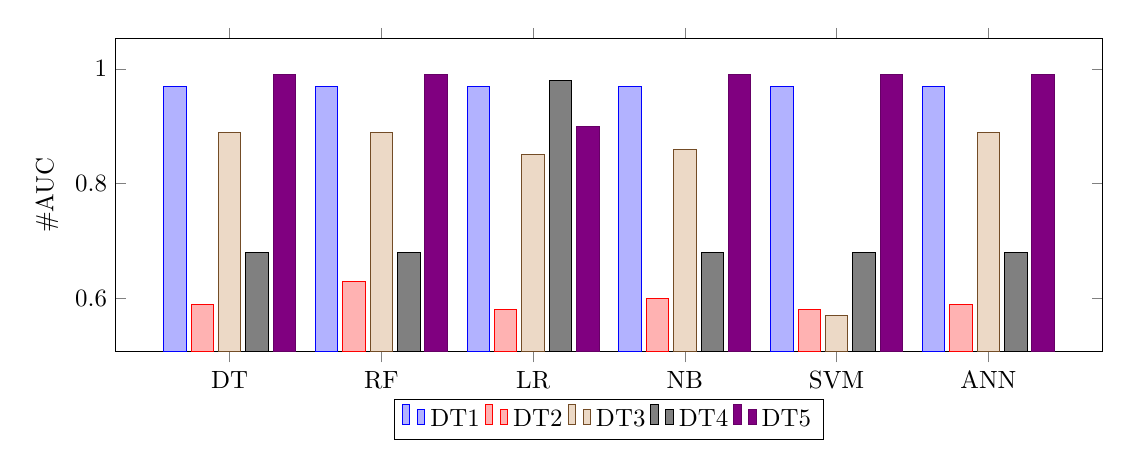
\begin{tikzpicture}[scale=0.9]
 %\centering
\begin{axis}[
     height=6cm, width=15.5cm,
    bar width=0.4cm,
    ybar,
    %ybar=5pt,% configures `bar shift'
    bar width=9pt,
    enlargelimits=0.15,
    legend style={at={(0.5,-0.15)},
    anchor=north,legend columns=-1},
    ylabel={\#AUC},
    symbolic x coords={{DT,RF,LR,NB,SVM,ANN}},
    xtick=data,
    %nodes near coords,
    nodes near coords align={vertical},
    ]
\addplot coordinates {(DT,0.97) (RF, 0.97) (LR,0.97)(NB, 0.97)(SVM,0.97)(ANN, 0.97)};
\addplot coordinates{(DT,0.59) (RF, 0.63) (LR,0.58)(NB, 0.60)(SVM,0.58)(ANN, 0.59)};
\addplot coordinates {(DT,0.89) (RF, 0.89) (LR,0.85)(NB, 0.86)(SVM,0.57)(ANN, 0.89)};
\addplot coordinates {(DT,0.68) (RF, 0.68) (LR,0.98)(NB, 0.68)(SVM,0.68)(ANN, 0.68)};
\addplot coordinates {(DT,0.99) (RF, 0.99) (LR,0.90)(NB, 0.99)(SVM,0.99)(ANN, 0.99)};
\legend{DT1,DT2,DT3,DT4,DT5}
\end{axis}
\end{tikzpicture}
%\caption{Precision values of compared classifiers on different datasets}

\end{figure}

\begin{figure}[h]
%\subfigure[Precison, F1-score, specificity values of the classifiers on DT1]{
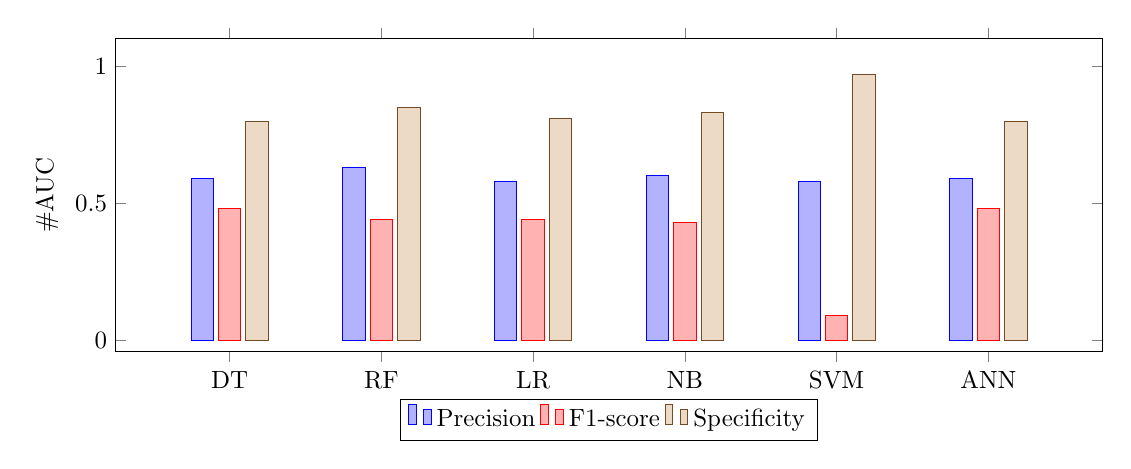
\begin{tikzpicture}[scale=0.9]
\begin{axis}[
     height=6cm, width=15.5cm,
    bar width=0.4cm,
    ybar,
    %ybar=5pt,% configures `bar shift'
    bar width=9pt,
    enlargelimits=0.15,
    legend style={at={(0.5,-0.15)},
    anchor=north,legend columns=-1},
    ylabel={\#AUC},
    symbolic x coords={{DT,RF,LR,NB,SVM,ANN}},
    xtick=data,
    %nodes near coords,
    nodes near coords align={vertical},
    ]
\addplot coordinates {(DT,0.59) (RF, 0.63) (LR,0.58)(NB, 0.60)(SVM,0.58)(ANN, 0.59)};
\addplot coordinates{(DT,0.48) (RF, 0.44) (LR,0.44)(NB, 0.43)(SVM,0.09)(ANN, 0.48)};
\addplot coordinates {(DT,0.80) (RF, 0.85) (LR,0.81)(NB, 0.83)(SVM,0.97)(ANN, 0.80)};
%\addplot coordinates {(DT,0.68) (RF, 0.68) (LR,0.98)(NB, 0.68)(SVM,0.68)(ANN, 0.68)};
%\addplot coordinates {(DT,0.99) (RF, 0.99) (LR,0.90)(NB, 0.99)(SVM,0.99)(ANN, 0.99)};
\legend{Precision,F1-score,Specificity,DT4}
\end{axis}
%\caption{Precison, F1-score, specificity values of the classifiers on DT1}
\end{tikzpicture}

\end{figure}